
%(BEGIN_QUESTION)
% Copyright 2007, Tony R. Kuphaldt, released under the Creative Commons Attribution License (v 1.0)
% This means you may do almost anything with this work of mine, so long as you give me proper credit

A ``bubbler'' or ``dip tube'' system may be used to transfer hydrostatic pressure from within a process vessel to some location outside the vessel, allowing a pressure-sensing instrument such as a gauge or transmitter to sense the liquid level inside the vessel without actually contacting the process liquid:

$$\includegraphics[width=15.5cm]{i02954x01.eps}$$

If the flow of purge air to the dip tube is slow, such that individual bubbles come out the end of the tube at a leisurely pace (one or two bubbles per second), the dip tube will function as a sort of ``pressure relief'' device.  At such a low flow rate, the air pressure within the dip tube almost exactly equalizes with the hydrostatic pressure of the liquid at the bottom of the tube.  Explain why this is, in your own words.

\vskip 10pt

Also, calculate the amount of pressure seen by the pressure gauge in this bubbler system, given a water height of 8 feet and 10 inches inside the vessel.  Assume the pressure regulator is set to 35 PSI.

\underbar{file i02954}
%(END_QUESTION)





%(BEGIN_ANSWER)

As compressed air slowly enters the dip tube, it presses the water out the bottom of the tube until the tube is dry.  At that point -- when all the water is pushed out the end of the tube -- the air pressure inside the tube precisely equals the hydrostatic pressure of the water at the bottom of the tube.

If the air pressure exceeds that hydrostatic water pressure by the slightest amount, an air bubble will escape from the tube's end.  As soon as this air bubble escapes, the pressure inside the tube drops back down to being precisely equal to the water's hydrostatic pressure.  In other words, at low air flow rates the water acts as a sort of pressure relief, preventing the air pressure from significantly exceeding the hydrostatic pressure.  In this way, the dip tube replicates the water's hydrostatic pressure in the form of air pressure, which may be sensed by any pressure-measuring instrument connected anywhere along the tube's length.

\vskip 10pt

$P_{gauge}$ = 3.829 PSI

%(END_ANSWER)





%(BEGIN_NOTES)

The regulator's pressure setting of 35 PSI is irrelevant to the dip tube air pressure calculation.  The regulator pressure need only be set to a level greater than the highest liquid level hydrostatic pressure in order for the bubbler system to function properly.

%INDEX% Measurement, level: bubble tube (bubbler)
%INDEX% Measurement, level: dip tube

%(END_NOTES)


